\SourceLeaf{214}\Needspace{18\baselineskip}
\begin{center}[2.]\end{center}

\begin{center}[CORRESPONDIRENDE PUNKTE IN PARALLELLINIEN.]\end{center}

1. \emph{\textls{Definition.}} \textls{Correspondirende Punkte in Parallellinien}, auf den gleichen Winkeln an der Verbindungslinie beruhend.

2. Sind $A$, $B$ correspondirende Punkte und $M$ in der Mitte von $AB$,

\begin{center}
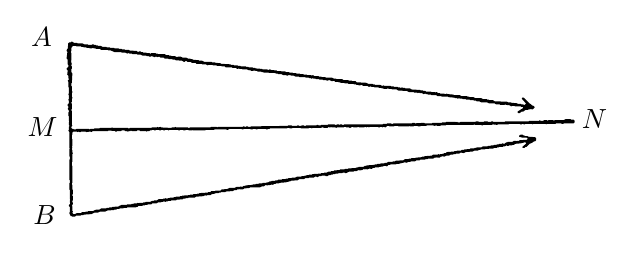
\begin{tikzpicture}[x=0.00650888cm,y=-0.00650888cm]
\fill[even odd rule] (106,393) -- (109,399) -- (111,399) -- (112,400) -- (117,400) -- (119,398) -- (128,398) -- (129,397) -- (133,397) -- (134,396) -- (149,395) -- (155,392) -- (162,392) -- (166,390) -- (176,390) -- (180,388) -- (193,387) -- (194,386) -- (198,386) -- (199,385) -- (203,385) -- (204,384) -- (211,384) -- (212,383) -- (218,383) -- (219,382) -- (236,382) -- (237,381) -- (239,381) -- (241,379) -- (248,379) -- (249,378) -- (253,378) -- (254,377) -- (258,377) -- (259,376) -- (266,376) -- (268,374) -- (276,374) -- (279,372) -- (285,372) -- (286,371) -- (289,371) -- (290,370) -- (294,371) -- (295,370) -- (298,370) -- (299,369) -- (304,369) -- (305,368) -- (314,368) -- (315,367) -- (327,366) -- (328,365) -- (332,365) -- (333,364) -- (337,364) -- (338,363) -- (350,363) -- (353,361) -- (367,360) -- (371,358) -- (373,359) -- (375,358) -- (381,358) -- (384,356) -- (390,355) -- (391,354) -- (397,354) -- (398,353) -- (401,353) -- (402,352) -- (410,352) -- (411,351) -- (425,350) -- (428,348) -- (432,348) -- (433,347) -- (436,347) -- (437,346) -- (439,347) -- (444,347) -- (447,345) -- (457,344) -- (458,343) -- (477,343) -- (481,341) -- (485,341) -- (489,338) -- (491,339) -- (499,338) -- (500,337) -- (503,338) -- (505,336) -- (508,336) -- (509,335) -- (515,335) -- (516,334) -- (529,333) -- (530,332) -- (533,332) -- (534,331) -- (537,331) -- (538,330) -- (551,329) -- (554,327) -- (563,327) -- (566,325) -- (572,325) -- (573,324) -- (582,324) -- (585,322) -- (588,322) -- (590,323) -- (593,321) -- (597,321) -- (598,320) -- (605,320) -- (606,321) -- (609,321) -- (612,319) -- (615,319) -- (616,318) -- (619,318) -- (620,317) -- (624,317) -- (625,316) -- (630,316) -- (631,315) -- (638,315) -- (639,314) -- (643,314) -- (644,315) -- (646,315) -- (652,312) -- (660,312) -- (661,311) -- (666,311) -- (670,309) -- (673,310) -- (674,309) -- (677,309) -- (680,307) -- (682,308) -- (684,307) -- (687,308) -- (691,306) -- (695,307) -- (698,305) -- (701,305) -- (702,304) -- (709,304) -- (710,303) -- (718,302) -- (719,301) -- (723,301) -- (725,302) -- (728,299) -- (731,299) -- (732,298) -- (743,298) -- (744,297) -- (749,297) -- (750,296) -- (753,296) -- (754,295) -- (757,295) -- (758,294) -- (761,294) -- (763,295) -- (764,294) -- (766,294) -- (767,293) -- (771,293) -- (772,292) -- (780,292) -- (783,290) -- (789,290) -- (790,289) -- (799,289) -- (800,288) -- (804,288) -- (805,287) -- (815,287) -- (818,285) -- (821,285) -- (822,284) -- (824,285) -- (828,285) -- (830,283) -- (832,283) -- (833,282) -- (837,283) -- (841,281) -- (846,281) -- (849,279) -- (854,279) -- (855,278) -- (859,278) -- (860,277) -- (866,277) -- (869,275) -- (875,276) -- (879,274) -- (892,273) -- (896,271) -- (903,271) -- (904,270) -- (907,270) -- (908,269) -- (916,269) -- (917,268) -- (933,267) -- (934,266) -- (939,266) -- (940,265) -- (943,265) -- (944,264) -- (951,264) -- (952,263) -- (955,263) -- (958,261) -- (960,262) -- (962,262) -- (963,261) -- (969,261) -- (970,260) -- (973,260) -- (975,258) -- (987,257) -- (988,256) -- (991,256) -- (992,255) -- (995,255) -- (997,257) -- (989,264) -- (990,266) -- (993,266) -- (995,264) -- (997,264) -- (1003,258) -- (1008,256) -- (1012,253) -- (1014,253) -- (1016,251) -- (1016,247) -- (1014,245) -- (1000,244) -- (999,243) -- (995,243) -- (994,242) -- (992,242) -- (989,240) -- (986,240) -- (983,242) -- (983,244) -- (984,245) -- (987,245) -- (988,246) -- (998,246) -- (1000,248) -- (998,250) -- (984,251) -- (983,252) -- (979,252) -- (978,253) -- (976,252) -- (973,252) -- (970,254) -- (961,254) -- (960,255) -- (958,255) -- (954,258) -- (950,257) -- (949,258) -- (944,258) -- (943,259) -- (940,259) -- (939,260) -- (934,260) -- (933,261) -- (928,261) -- (927,262) -- (922,262) -- (921,263) -- (912,263) -- (909,265) -- (900,265) -- (899,266) -- (896,266) -- (895,267) -- (888,267) -- (887,268) -- (876,269) -- (875,270) -- (871,270) -- (870,271) -- (862,271) -- (861,272) -- (857,272) -- (856,273) -- (842,274) -- (840,276) -- (837,276) -- (836,277) -- (834,277) -- (833,278) -- (829,278) -- (828,279) -- (826,278) -- (824,279) -- (815,279) -- (813,281) -- (799,282) -- (798,283) -- (794,283) -- (793,284) -- (781,285) -- (780,286) -- (773,286) -- (772,287) -- (768,287) -- (767,288) -- (760,288) -- (757,290) -- (742,291) -- (741,292) -- (737,292) -- (736,293) -- (728,293) -- (725,295) -- (721,295) -- (720,296) -- (713,296) -- (712,297) -- (707,297) -- (706,298) -- (702,298) -- (701,299) -- (686,300) -- (685,301) -- (682,301) -- (679,303) -- (670,303) -- (669,304) -- (666,304) -- (665,305) -- (650,306) -- (649,307) -- (643,307) -- (642,308) -- (634,308) -- (633,309) -- (622,310) -- (621,311) -- (617,311) -- (616,312) -- (612,312) -- (608,314) -- (603,314) -- (602,315) -- (597,315) -- (596,316) -- (580,317) -- (579,318) -- (574,318) -- (573,319) -- (569,319) -- (568,320) -- (565,320) -- (564,321) -- (559,321) -- (558,322) -- (550,322) -- (546,324) -- (540,324) -- (539,325) -- (533,325) -- (532,326) -- (528,326) -- (527,327) -- (521,327) -- (520,328) -- (513,328) -- (512,329) -- (508,329) -- (507,330) -- (501,330) -- (500,331) -- (497,331) -- (494,333) -- (491,333) -- (490,334) -- (483,334) -- (482,335) -- (476,335) -- (475,336) -- (470,336) -- (469,337) -- (464,337) -- (463,338) -- (450,339) -- (449,340) -- (446,340) -- (443,342) -- (440,341) -- (439,342) -- (432,342) -- (428,344) -- (418,344) -- (414,346) -- (403,347) -- (401,349) -- (391,349) -- (390,350) -- (383,350) -- (381,352) -- (377,352) -- (376,353) -- (360,354) -- (359,355) -- (356,355) -- (355,356) -- (348,356) -- (347,357) -- (342,357) -- (341,358) -- (326,359) -- (325,360) -- (322,360) -- (321,361) -- (314,361) -- (313,362) -- (310,362) -- (309,363) -- (302,363) -- (301,364) -- (298,364) -- (297,365) -- (293,364) -- (292,365) -- (289,365) -- (288,366) -- (280,366) -- (277,368) -- (272,368) -- (271,369) -- (268,369) -- (264,371) -- (255,371) -- (254,372) -- (251,372) -- (250,373) -- (243,373) -- (242,374) -- (239,373) -- (238,374) -- (232,374) -- (231,375) -- (228,375) -- (227,376) -- (219,376) -- (218,377) -- (208,377) -- (207,378) -- (205,378) -- (203,380) -- (190,381) -- (189,382) -- (184,382) -- (183,383) -- (179,383) -- (178,384) -- (168,384) -- (165,386) -- (159,386) -- (152,389) -- (143,389) -- (142,390) -- (138,390) -- (137,391) -- (131,391) -- (129,393) -- (121,393) -- (117,395) -- (114,395) -- (112,393) -- (113,390) -- (112,389) -- (112,380) -- (111,379) -- (113,375) -- (113,373) -- (112,372) -- (112,369) -- (113,368) -- (113,360) -- (112,359) -- (112,357) -- (113,356) -- (113,348) -- (112,347) -- (112,338) -- (111,337) -- (111,335) -- (112,334) -- (112,301) -- (111,300) -- (111,294) -- (112,293) -- (112,278) -- (113,276) -- (112,275) -- (112,270) -- (111,269) -- (111,267) -- (112,266) -- (111,264) -- (112,262) -- (112,249) -- (111,248) -- (111,241) -- (112,240) -- (112,236) -- (114,234) -- (121,234) -- (122,235) -- (124,234) -- (126,235) -- (128,235) -- (129,234) -- (138,234) -- (139,235) -- (147,234) -- (149,235) -- (152,233) -- (181,233) -- (182,232) -- (195,233) -- (196,234) -- (198,234) -- (199,233) -- (207,233) -- (208,232) -- (214,232) -- (215,233) -- (218,233) -- (219,234) -- (225,233) -- (226,232) -- (228,233) -- (237,233) -- (238,232) -- (243,232) -- (244,233) -- (255,233) -- (257,234) -- (258,233) -- (262,233) -- (263,232) -- (266,232) -- (267,231) -- (271,231) -- (272,232) -- (274,232) -- (275,231) -- (281,231) -- (282,232) -- (284,232) -- (285,231) -- (289,231) -- (290,232) -- (292,232) -- (293,231) -- (298,231) -- (299,232) -- (301,231) -- (318,231) -- (319,232) -- (321,232) -- (322,231) -- (328,231) -- (329,232) -- (332,232) -- (333,231) -- (338,231) -- (339,232) -- (345,232) -- (346,231) -- (348,232) -- (371,232) -- (372,231) -- (388,231) -- (389,230) -- (412,230) -- (414,231) -- (418,229) -- (442,229) -- (443,230) -- (445,230) -- (446,229) -- (459,229) -- (460,230) -- (463,230) -- (464,229) -- (469,229) -- (470,230) -- (472,230) -- (473,229) -- (489,229) -- (490,230) -- (492,230) -- (493,229) -- (496,229) -- (497,228) -- (530,228) -- (531,227) -- (535,227) -- (536,228) -- (540,228) -- (541,227) -- (557,227) -- (558,228) -- (572,228) -- (573,227) -- (577,227) -- (579,228) -- (580,227) -- (597,227) -- (598,226) -- (601,226) -- (602,227) -- (609,227) -- (611,225) -- (613,226) -- (615,226) -- (616,225) -- (618,226) -- (625,226) -- (626,227) -- (628,226) -- (641,226) -- (642,225) -- (645,225) -- (646,226) -- (651,226) -- (653,227) -- (657,225) -- (659,225) -- (660,226) -- (667,226) -- (668,225) -- (670,225) -- (671,226) -- (681,226) -- (682,225) -- (684,225) -- (685,226) -- (687,225) -- (689,225) -- (690,226) -- (692,225) -- (708,225) -- (709,226) -- (711,226) -- (712,225) -- (715,225) -- (717,226) -- (718,225) -- (720,225) -- (722,226) -- (726,223) -- (729,223) -- (730,224) -- (739,224) -- (740,223) -- (747,223) -- (748,224) -- (768,224) -- (769,223) -- (771,224) -- (777,224) -- (778,223) -- (785,223) -- (786,224) -- (790,224) -- (791,223) -- (802,223) -- (803,222) -- (816,222) -- (817,223) -- (822,222) -- (823,223) -- (829,223) -- (830,222) -- (840,222) -- (841,221) -- (894,221) -- (895,220) -- (897,221) -- (909,221) -- (910,222) -- (912,222) -- (913,221) -- (930,221) -- (931,220) -- (940,221) -- (941,220) -- (962,220) -- (963,219) -- (984,219) -- (985,220) -- (988,220) -- (989,219) -- (991,219) -- (992,220) -- (994,220) -- (995,219) -- (1008,219) -- (1009,220) -- (1011,219) -- (1034,219) -- (1036,220) -- (1037,219) -- (1054,219) -- (1055,218) -- (1065,218) -- (1066,219) -- (1069,219) -- (1070,218) -- (1089,218) -- (1091,216) -- (1091,213) -- (1089,211) -- (1084,211) -- (1083,210) -- (1073,210) -- (1069,212) -- (1052,212) -- (1051,213) -- (1049,212) -- (1040,212) -- (1039,213) -- (1037,212) -- (1031,212) -- (1030,213) -- (1025,213) -- (1023,212) -- (1022,213) -- (1003,213) -- (1002,214) -- (956,214) -- (955,215) -- (932,215) -- (931,214) -- (929,214) -- (928,215) -- (922,215) -- (921,214) -- (915,214) -- (914,215) -- (904,215) -- (903,214) -- (899,214) -- (898,215) -- (869,215) -- (868,216) -- (863,216) -- (862,215) -- (860,216) -- (858,215) -- (841,215) -- (840,216) -- (833,216) -- (832,217) -- (814,217) -- (813,218) -- (799,218) -- (798,217) -- (780,218) -- (779,217) -- (775,217) -- (774,218) -- (738,218) -- (737,219) -- (734,219) -- (733,218) -- (726,218) -- (725,219) -- (718,219) -- (717,220) -- (642,220) -- (641,221) -- (638,221) -- (637,220) -- (634,220) -- (633,221) -- (631,220) -- (628,220) -- (627,221) -- (624,221) -- (623,220) -- (611,220) -- (610,221) -- (597,221) -- (596,222) -- (592,222) -- (591,221) -- (589,221) -- (588,222) -- (568,222) -- (567,223) -- (564,223) -- (563,222) -- (559,222) -- (558,223) -- (554,223) -- (553,222) -- (551,222) -- (550,223) -- (540,223) -- (539,222) -- (533,222) -- (532,223) -- (460,224) -- (459,225) -- (455,225) -- (454,224) -- (451,224) -- (450,225) -- (448,225) -- (447,224) -- (445,224) -- (444,225) -- (396,225) -- (395,226) -- (393,225) -- (382,225) -- (381,226) -- (341,226) -- (340,227) -- (338,227) -- (337,226) -- (314,226) -- (313,225) -- (311,226) -- (306,226) -- (305,227) -- (285,226) -- (284,225) -- (280,226) -- (278,225) -- (277,226) -- (267,226) -- (266,227) -- (224,227) -- (223,228) -- (221,228) -- (220,227) -- (191,227) -- (189,226) -- (188,227) -- (166,227) -- (165,228) -- (155,228) -- (154,229) -- (147,229) -- (146,230) -- (144,229) -- (120,229) -- (119,230) -- (115,230) -- (114,229) -- (112,229) -- (110,227) -- (110,225) -- (112,223) -- (111,221) -- (111,194) -- (110,193) -- (110,191) -- (111,190) -- (111,180) -- (110,179) -- (110,177) -- (111,176) -- (111,170) -- (112,169) -- (112,167) -- (111,166) -- (111,159) -- (112,158) -- (112,156) -- (111,155) -- (111,146) -- (110,145) -- (110,140) -- (111,139) -- (112,121) -- (110,118) -- (110,112) -- (111,111) -- (111,107) -- (110,106) -- (110,104) -- (111,102) -- (110,101) -- (110,98) -- (109,97) -- (110,95) -- (110,81) -- (109,80) -- (109,78) -- (110,77) -- (110,71) -- (113,67) -- (119,67) -- (120,68) -- (129,68) -- (130,69) -- (133,69) -- (134,70) -- (139,70) -- (140,71) -- (145,71) -- (146,72) -- (150,72) -- (151,71) -- (153,71) -- (154,72) -- (157,72) -- (158,73) -- (166,73) -- (168,75) -- (181,75) -- (182,76) -- (187,76) -- (194,79) -- (207,79) -- (208,80) -- (215,80) -- (219,82) -- (222,81) -- (223,82) -- (228,82) -- (229,83) -- (238,83) -- (239,84) -- (245,84) -- (249,86) -- (256,86) -- (257,87) -- (261,87) -- (262,88) -- (265,88) -- (266,87) -- (270,88) -- (271,89) -- (273,89) -- (274,88) -- (276,88) -- (277,89) -- (281,88) -- (284,90) -- (290,90) -- (292,92) -- (299,92) -- (300,93) -- (307,93) -- (308,94) -- (312,94) -- (313,95) -- (326,96) -- (329,98) -- (331,98) -- (332,97) -- (335,97) -- (336,98) -- (342,98) -- (345,100) -- (352,100) -- (354,102) -- (364,102) -- (365,103) -- (372,103) -- (376,105) -- (378,104) -- (385,104) -- (386,105) -- (393,105) -- (394,106) -- (402,106) -- (403,107) -- (409,107) -- (411,109) -- (423,109) -- (424,110) -- (431,110) -- (433,112) -- (437,111) -- (438,112) -- (443,112) -- (444,113) -- (453,113) -- (454,114) -- (460,115) -- (461,116) -- (468,115) -- (469,116) -- (472,116) -- (473,117) -- (480,117) -- (481,118) -- (484,118) -- (485,119) -- (508,120) -- (509,121) -- (512,121) -- (513,122) -- (519,122) -- (523,124) -- (529,124) -- (530,125) -- (532,125) -- (533,124) -- (537,124) -- (538,125) -- (543,125) -- (547,127) -- (554,127) -- (555,128) -- (566,128) -- (567,129) -- (573,129) -- (574,130) -- (577,130) -- (578,131) -- (581,130) -- (582,131) -- (586,131) -- (587,132) -- (593,132) -- (594,133) -- (600,133) -- (601,134) -- (607,134) -- (608,135) -- (610,135) -- (611,134) -- (614,134) -- (618,136) -- (622,135) -- (624,137) -- (630,137) -- (631,138) -- (634,138) -- (635,139) -- (642,139) -- (643,140) -- (649,140) -- (650,141) -- (660,141) -- (661,142) -- (665,142) -- (666,143) -- (669,143) -- (670,144) -- (673,144) -- (675,143) -- (679,145) -- (687,145) -- (690,147) -- (694,146) -- (695,147) -- (700,147) -- (701,148) -- (709,148) -- (710,149) -- (714,149) -- (715,150) -- (718,150) -- (719,151) -- (725,151) -- (726,150) -- (728,150) -- (729,151) -- (734,151) -- (735,152) -- (744,152) -- (747,154) -- (764,155) -- (768,157) -- (777,157) -- (778,158) -- (784,158) -- (785,159) -- (788,158) -- (789,159) -- (794,159) -- (796,161) -- (800,160) -- (801,161) -- (804,161) -- (805,162) -- (811,162) -- (812,163) -- (821,163) -- (824,165) -- (831,165) -- (832,166) -- (844,166) -- (845,167) -- (857,168) -- (858,169) -- (862,169) -- (863,170) -- (866,169) -- (867,170) -- (872,170) -- (873,171) -- (879,171) -- (880,172) -- (887,172) -- (888,173) -- (894,173) -- (895,174) -- (899,174) -- (900,175) -- (905,175) -- (909,177) -- (920,177) -- (924,179) -- (935,179) -- (938,181) -- (945,181) -- (946,182) -- (954,182) -- (956,181) -- (957,182) -- (965,183) -- (967,185) -- (969,184) -- (974,184) -- (975,185) -- (986,185) -- (987,186) -- (990,186) -- (991,188) -- (980,195) -- (980,197) -- (981,198) -- (984,198) -- (988,195) -- (991,195) -- (995,192) -- (1000,192) -- (1001,191) -- (1004,191) -- (1005,190) -- (1009,191) -- (1013,187) -- (1013,186) -- (1011,184) -- (1008,183) -- (1005,180) -- (1004,180) -- (992,168) -- (989,168) -- (988,170) -- (996,179) -- (996,180) -- (994,182) -- (992,182) -- (991,181) -- (987,181) -- (986,180) -- (980,180) -- (979,179) -- (968,178) -- (967,177) -- (961,177) -- (960,176) -- (935,175) -- (932,173) -- (925,173) -- (924,172) -- (921,172) -- (920,171) -- (913,171) -- (909,169) -- (898,169) -- (894,167) -- (886,167) -- (885,166) -- (882,166) -- (881,165) -- (871,165) -- (867,163) -- (856,163) -- (855,162) -- (843,161) -- (842,160) -- (840,161) -- (838,161) -- (837,160) -- (829,160) -- (828,159) -- (825,159) -- (822,157) -- (819,158) -- (818,157) -- (812,157) -- (811,156) -- (801,156) -- (800,155) -- (796,155) -- (795,154) -- (791,154) -- (790,153) -- (773,152) -- (770,150) -- (761,150) -- (760,149) -- (756,149) -- (755,148) -- (751,149) -- (750,148) -- (747,148) -- (746,147) -- (739,147) -- (738,146) -- (733,146) -- (732,145) -- (720,145) -- (719,144) -- (716,145) -- (712,143) -- (702,143) -- (701,142) -- (698,142) -- (697,141) -- (689,141) -- (685,139) -- (666,138) -- (664,136) -- (658,136) -- (657,135) -- (651,135) -- (650,134) -- (641,134) -- (638,132) -- (627,132) -- (626,131) -- (622,131) -- (618,129) -- (606,129) -- (605,128) -- (598,128) -- (597,127) -- (593,127) -- (592,126) -- (584,126) -- (581,124) -- (579,125) -- (577,124) -- (570,124) -- (569,123) -- (563,123) -- (562,122) -- (556,122) -- (555,121) -- (549,121) -- (548,120) -- (542,120) -- (541,119) -- (535,119) -- (534,118) -- (528,118) -- (527,117) -- (511,116) -- (510,115) -- (499,114) -- (498,113) -- (496,113) -- (495,114) -- (493,114) -- (492,113) -- (483,113) -- (482,112) -- (469,111) -- (468,110) -- (464,110) -- (463,109) -- (456,109) -- (455,108) -- (451,108) -- (450,107) -- (440,107) -- (439,106) -- (435,106) -- (434,105) -- (427,105) -- (426,104) -- (421,104) -- (420,103) -- (402,102) -- (401,101) -- (391,100) -- (390,99) -- (384,99) -- (383,98) -- (369,98) -- (365,96) -- (359,96) -- (358,95) -- (347,94) -- (346,93) -- (343,93) -- (342,92) -- (338,92) -- (334,90) -- (327,90) -- (323,88) -- (318,88) -- (316,89) -- (312,87) -- (305,87) -- (304,86) -- (301,86) -- (300,85) -- (295,85) -- (292,83) -- (279,83) -- (278,82) -- (275,82) -- (274,81) -- (266,81) -- (265,82) -- (263,82) -- (262,81) -- (257,81) -- (256,80) -- (250,80) -- (249,79) -- (246,79) -- (245,78) -- (242,78) -- (240,79) -- (237,77) -- (223,76) -- (222,75) -- (215,75) -- (214,74) -- (209,74) -- (208,73) -- (203,73) -- (202,72) -- (194,72) -- (193,71) -- (186,71) -- (185,70) -- (179,70) -- (178,69) -- (171,69) -- (167,67) -- (162,67) -- (161,66) -- (158,66) -- (157,65) -- (154,65) -- (153,64) -- (151,64) -- (150,65) -- (143,65) -- (142,64) -- (135,64) -- (131,62) -- (122,62) -- (121,61) -- (115,61) -- (112,59) -- (110,59) -- (109,60) -- (106,60) -- (104,62) -- (103,72) -- (101,75) -- (101,77) -- (103,79) -- (102,81) -- (102,85) -- (101,86) -- (102,87) -- (101,88) -- (101,92) -- (103,94) -- (103,103) -- (104,104) -- (104,108) -- (101,111) -- (101,113) -- (103,115) -- (102,123) -- (104,125) -- (104,130) -- (105,131) -- (105,133) -- (103,135) -- (104,137) -- (104,147) -- (105,148) -- (105,160) -- (104,161) -- (105,163) -- (105,171) -- (104,172) -- (105,174) -- (105,179) -- (103,181) -- (103,184) -- (104,185) -- (104,188) -- (103,190) -- (105,193) -- (105,196) -- (104,197) -- (104,203) -- (105,204) -- (105,213) -- (106,214) -- (105,216) -- (105,221) -- (106,222) -- (106,224) -- (105,225) -- (105,231) -- (104,232) -- (106,235) -- (106,266) -- (107,267) -- (106,269) -- (106,282) -- (107,283) -- (107,288) -- (106,289) -- (106,328) -- (107,329) -- (107,334) -- (106,335) -- (106,347) -- (107,348) -- (107,366) -- (108,367) -- (107,369) -- (107,372) -- (108,374) -- (105,378) -- (105,379) -- (107,381) -- (107,391) -- cycle;
\node[inner sep=0pt] at (52,50) {$A$};
\node[inner sep=0pt] at (1130,210) {$N$};
\node[inner sep=0pt] at (54,226) {$M$};
\node[inner sep=0pt] at (58,397) {$B$};
\end{tikzpicture}

\end{center}
\noindent $MN$ senkrecht auf $AB$, so wird 1) $MN$ mit beiden parallel sein, 2) jeder Punkt, welcher mit $A$ auf Einer Seite von $MN$ liegt, wird dem $A$ näher sein als [dem] $B$.

.\ .\ .\ .\ .\ .\ .\ .\ .\ .\ .\ . 

4. \emph{Theorem.} Sind $A$, $B$ correspondirende Punkte auf den Parallelen $1$, $2$ und $A'$, $B'$ desgleichen, so ist $AA' = BB'$ und vice versa.

\Needspace{16\baselineskip}
5. \emph{Theorem.} Sind $A$, $B$, $C$ Punkte auf den Parallelen $1$, $2$, $3$ und $A$ mit $B$, $B$ mit $C$ correspondirend; so ist auch $A$ mit $C$ correspondirend.

\textls{Beweis.} Im entgegengesetzten Fall sei der Winkel $C > A$; man nehme

\begin{center}
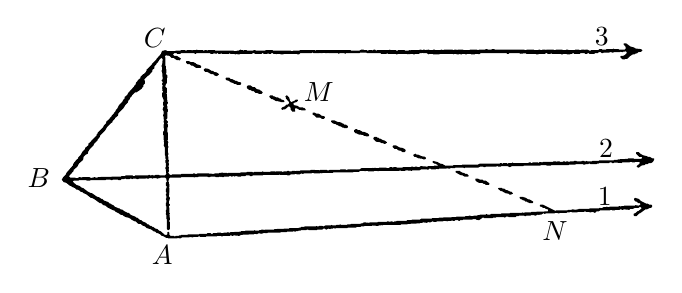
\begin{tikzpicture}[x=0.00661355cm,y=-0.00661355cm]
\fill[even odd rule] (968,355) -- (968,356) -- (971,359) -- (973,359) -- (975,361) -- (977,361) -- (979,363) -- (982,363) -- (984,365) -- (986,365) -- (987,366) -- (993,366) -- (994,365) -- (994,363) -- (987,359) -- (985,359) -- (978,355) -- (976,355) -- (975,354) -- (969,354) -- cycle
(927,338) -- (927,339) -- (932,343) -- (934,343) -- (941,347) -- (947,348) -- (949,350) -- (951,350) -- (955,348) -- (955,347) -- (952,344) -- (950,344) -- (944,341) -- (942,341) -- (938,338) -- (935,338) -- (934,337) -- (928,337) -- cycle
(883,320) -- (883,322) -- (886,325) -- (890,327) -- (896,327) -- (899,329) -- (901,329) -- (903,331) -- (909,331) -- (910,330) -- (910,328) -- (903,323) -- (899,323) -- (897,321) -- (892,321) -- (888,319) -- (884,319) -- cycle
(845,305) -- (845,307) -- (854,312) -- (859,313) -- (862,315) -- (869,315) -- (870,314) -- (870,313) -- (867,310) -- (864,310) -- (861,308) -- (859,308) -- (855,306) -- (853,304) -- (846,304) -- cycle
(764,273) -- (764,275) -- (766,277) -- (768,277) -- (774,280) -- (782,281) -- (783,282) -- (786,282) -- (788,280) -- (788,279) -- (786,277) -- (780,276) -- (773,273) -- (770,273) -- (768,271) -- cycle
(724,257) -- (724,258) -- (728,262) -- (732,262) -- (734,264) -- (736,265) -- (739,265) -- (743,268) -- (747,268) -- (749,266) -- (749,264) -- (747,262) -- (743,260) -- (737,259) -- (730,255) -- (726,255) -- cycle
(687,241) -- (687,243) -- (692,248) -- (700,249) -- (703,251) -- (706,251) -- (707,252) -- (710,252) -- (713,250) -- (713,249) -- (709,246) -- (705,245) -- (700,242) -- (698,242) -- (696,240) -- (694,240) -- (693,239) -- (689,239) -- cycle
(650,226) -- (650,229) -- (653,232) -- (655,232) -- (658,234) -- (667,235) -- (669,237) -- (672,237) -- (673,238) -- (677,238) -- (679,236) -- (679,235) -- (676,232) -- (669,229) -- (666,229) -- (661,226) -- (658,226) -- (655,224) -- (653,224) -- cycle
(606,208) -- (606,210) -- (608,212) -- (612,214) -- (614,214) -- (617,216) -- (619,216) -- (621,218) -- (625,219) -- (628,221) -- (630,221) -- (631,222) -- (636,222) -- (638,220) -- (638,218) -- (637,217) -- (636,217) -- (634,215) -- (631,215) -- (629,213) -- (627,213) -- (625,211) -- (618,210) -- (612,207) -- (607,207) -- cycle
(570,193) -- (570,196) -- (574,198) -- (578,202) -- (585,202) -- (588,204) -- (592,204) -- (594,202) -- (594,201) -- (592,199) -- (587,198) -- (585,196) -- (581,194) -- (577,194) -- (574,192) -- (571,192) -- cycle
(510,184) -- (510,185) -- (512,187) -- (514,186) -- (517,186) -- (524,180) -- (525,180) -- (528,183) -- (528,186) -- (531,190) -- (536,190) -- (537,189) -- (536,187) -- (536,185) -- (537,184) -- (540,184) -- (545,187) -- (548,187) -- (549,188) -- (556,188) -- (557,187) -- (557,186) -- (554,183) -- (552,183) -- (551,182) -- (545,182) -- (541,179) -- (535,178) -- (533,176) -- (533,175) -- (535,173) -- (539,172) -- (542,169) -- (542,168) -- (541,167) -- (538,167) -- (536,169) -- (529,172) -- (527,170) -- (525,163) -- (521,159) -- (520,159) -- (518,161) -- (518,162) -- (519,163) -- (519,165) -- (525,172) -- (525,174) -- (522,177) -- (520,177) -- (517,180) -- (512,182) -- cycle
(487,161) -- (487,162) -- (491,166) -- (493,166) -- (500,170) -- (504,170) -- (505,171) -- (508,171) -- (509,172) -- (515,172) -- (516,171) -- (516,170) -- (514,168) -- (510,167) -- (508,165) -- (506,165) -- (504,163) -- (500,163) -- (497,161) -- (495,161) -- (493,159) -- (489,159) -- cycle
(444,142) -- (444,145) -- (446,147) -- (450,149) -- (452,149) -- (454,151) -- (457,151) -- (460,154) -- (463,154) -- (467,156) -- (472,156) -- (474,154) -- (474,153) -- (471,150) -- (470,150) -- (468,148) -- (463,147) -- (459,143) -- (455,143) -- (451,140) -- (446,140) -- cycle
(403,126) -- (403,128) -- (405,130) -- (409,131) -- (413,134) -- (417,135) -- (420,137) -- (422,137) -- (426,139) -- (431,139) -- (433,137) -- (433,135) -- (432,134) -- (427,133) -- (424,131) -- (422,131) -- (416,128) -- (413,128) -- (410,125) -- (404,125) -- cycle
(361,109) -- (361,111) -- (364,114) -- (368,114) -- (375,118) -- (379,118) -- (382,121) -- (386,122) -- (390,119) -- (390,118) -- (386,115) -- (381,114) -- (379,112) -- (376,112) -- (370,108) -- (364,107) -- cycle
(327,94) -- (327,96) -- (330,99) -- (334,99) -- (337,102) -- (340,102) -- (346,106) -- (355,106) -- (356,105) -- (356,103) -- (354,101) -- (347,99) -- (345,97) -- (341,95) -- (336,95) -- (332,93) -- (328,93) -- cycle
(1204,72) -- (1201,70) -- (1191,69) -- (1188,67) -- (1181,65) -- (1173,59) -- (1169,59) -- (1168,60) -- (1168,61) -- (1172,66) -- (1172,69) -- (1170,71) -- (1159,71) -- (1158,70) -- (1150,70) -- (1148,69) -- (1147,70) -- (1135,70) -- (1134,71) -- (1127,71) -- (1126,70) -- (1122,70) -- (1119,72) -- (1106,72) -- (1105,73) -- (1102,73) -- (1098,71) -- (1095,71) -- (1094,72) -- (1092,71) -- (1087,71) -- (1086,72) -- (1083,72) -- (1082,71) -- (1075,71) -- (1074,72) -- (1062,72) -- (1061,71) -- (1058,71) -- (1057,72) -- (1051,72) -- (1050,71) -- (1038,71) -- (1037,72) -- (1034,72) -- (1033,71) -- (1020,71) -- (1019,72) -- (1017,71) -- (1012,71) -- (1011,72) -- (1008,72) -- (1007,71) -- (1005,71) -- (1004,72) -- (996,72) -- (995,71) -- (982,71) -- (981,72) -- (978,72) -- (977,71) -- (920,71) -- (919,70) -- (915,70) -- (914,71) -- (907,71) -- (906,70) -- (903,70) -- (902,71) -- (890,71) -- (889,72) -- (887,72) -- (886,71) -- (873,71) -- (872,72) -- (860,72) -- (859,71) -- (849,71) -- (848,72) -- (846,71) -- (843,71) -- (842,72) -- (840,72) -- (839,71) -- (823,71) -- (822,72) -- (820,72) -- (819,71) -- (817,71) -- (816,72) -- (806,72) -- (805,71) -- (802,71) -- (801,72) -- (795,72) -- (794,71) -- (786,72) -- (785,71) -- (783,71) -- (782,72) -- (780,72) -- (779,71) -- (776,71) -- (775,72) -- (759,72) -- (758,73) -- (756,72) -- (754,73) -- (748,73) -- (747,72) -- (735,72) -- (734,73) -- (731,73) -- (730,72) -- (720,72) -- (719,71) -- (717,72) -- (694,72) -- (693,73) -- (692,73) -- (690,71) -- (688,71) -- (686,73) -- (684,72) -- (678,72) -- (677,73) -- (675,73) -- (674,72) -- (669,72) -- (668,71) -- (664,71) -- (660,73) -- (644,73) -- (643,72) -- (577,72) -- (576,73) -- (574,72) -- (546,72) -- (545,73) -- (533,73) -- (532,74) -- (529,74) -- (528,73) -- (494,73) -- (493,72) -- (480,72) -- (479,73) -- (461,73) -- (460,72) -- (457,72) -- (456,73) -- (444,73) -- (443,72) -- (439,72) -- (437,73) -- (436,72) -- (433,72) -- (432,71) -- (428,73) -- (425,73) -- (424,74) -- (419,74) -- (418,73) -- (383,73) -- (382,72) -- (369,72) -- (368,73) -- (366,72) -- (363,72) -- (362,73) -- (360,73) -- (359,72) -- (349,72) -- (348,71) -- (346,72) -- (340,72) -- (339,73) -- (337,72) -- (329,72) -- (328,73) -- (326,73) -- (325,72) -- (317,72) -- (316,73) -- (307,73) -- (306,74) -- (291,74) -- (290,73) -- (286,72) -- (285,73) -- (282,73) -- (280,75) -- (279,79) -- (270,89) -- (270,90) -- (261,99) -- (261,100) -- (253,108) -- (251,109) -- (251,111) -- (249,115) -- (246,118) -- (245,118) -- (239,124) -- (239,126) -- (234,130) -- (234,131) -- (231,134) -- (230,138) -- (227,141) -- (227,142) -- (216,154) -- (214,158) -- (209,162) -- (209,165) -- (206,168) -- (204,172) -- (198,178) -- (195,184) -- (192,187) -- (191,190) -- (188,193) -- (188,194) -- (184,198) -- (184,199) -- (180,203) -- (180,204) -- (174,209) -- (173,213) -- (169,217) -- (167,221) -- (157,231) -- (157,232) -- (155,234) -- (155,236) -- (144,247) -- (144,248) -- (139,252) -- (139,255) -- (133,260) -- (133,262) -- (128,267) -- (124,274) -- (120,278) -- (119,281) -- (117,282) -- (112,288) -- (112,289) -- (110,291) -- (110,293) -- (97,308) -- (96,311) -- (91,316) -- (88,321) -- (92,326) -- (94,326) -- (98,328) -- (104,333) -- (106,333) -- (108,335) -- (113,337) -- (116,340) -- (118,340) -- (122,342) -- (124,344) -- (128,345) -- (130,347) -- (135,349) -- (144,356) -- (146,356) -- (150,358) -- (161,366) -- (164,366) -- (168,370) -- (172,371) -- (177,375) -- (187,380) -- (189,380) -- (192,383) -- (198,386) -- (200,388) -- (205,389) -- (207,391) -- (211,393) -- (216,394) -- (220,396) -- (222,398) -- (228,401) -- (230,401) -- (234,405) -- (236,406) -- (240,406) -- (243,409) -- (248,411) -- (251,414) -- (258,416) -- (262,418) -- (264,420) -- (268,421) -- (271,424) -- (273,424) -- (277,426) -- (280,429) -- (282,429) -- (289,433) -- (292,433) -- (293,434) -- (310,434) -- (311,433) -- (316,434) -- (319,432) -- (333,432) -- (334,431) -- (340,432) -- (341,431) -- (350,431) -- (351,430) -- (353,430) -- (354,431) -- (365,431) -- (366,430) -- (386,430) -- (387,429) -- (394,429) -- (395,430) -- (397,430) -- (398,429) -- (411,429) -- (412,428) -- (414,428) -- (415,429) -- (417,429) -- (418,428) -- (429,429) -- (433,427) -- (457,426) -- (458,425) -- (461,425) -- (463,426) -- (466,424) -- (473,425) -- (474,424) -- (477,424) -- (478,423) -- (480,424) -- (483,424) -- (484,423) -- (508,423) -- (509,422) -- (520,422) -- (521,421) -- (532,421) -- (533,420) -- (537,421) -- (538,420) -- (542,420) -- (543,419) -- (547,419) -- (548,418) -- (558,418) -- (559,417) -- (562,417) -- (563,418) -- (578,418) -- (579,417) -- (589,417) -- (591,415) -- (594,415) -- (596,417) -- (597,417) -- (600,415) -- (604,416) -- (605,415) -- (609,415) -- (610,414) -- (614,415) -- (615,414) -- (637,414) -- (638,413) -- (654,413) -- (655,412) -- (662,412) -- (663,411) -- (669,411) -- (670,410) -- (684,410) -- (685,409) -- (696,410) -- (697,409) -- (701,409) -- (702,408) -- (704,409) -- (706,408) -- (739,408) -- (740,407) -- (752,407) -- (753,406) -- (776,405) -- (777,404) -- (781,404) -- (782,403) -- (790,404) -- (792,402) -- (794,403) -- (797,403) -- (801,401) -- (803,402) -- (808,402) -- (809,401) -- (821,401) -- (822,400) -- (830,401) -- (831,400) -- (837,400) -- (838,399) -- (840,400) -- (843,400) -- (844,399) -- (850,399) -- (851,400) -- (853,400) -- (854,399) -- (858,399) -- (859,398) -- (877,398) -- (878,397) -- (884,397) -- (885,398) -- (890,399) -- (897,394) -- (899,394) -- (900,395) -- (916,395) -- (917,394) -- (922,394) -- (923,393) -- (938,393) -- (940,394) -- (942,392) -- (946,392) -- (947,393) -- (960,393) -- (962,391) -- (966,391) -- (967,390) -- (977,390) -- (978,391) -- (980,391) -- (981,390) -- (989,390) -- (990,389) -- (996,389) -- (997,390) -- (999,390) -- (1003,388) -- (1005,389) -- (1007,388) -- (1010,388) -- (1013,386) -- (1015,386) -- (1016,387) -- (1018,386) -- (1035,386) -- (1036,385) -- (1041,385) -- (1042,386) -- (1044,386) -- (1045,385) -- (1058,385) -- (1059,384) -- (1064,384) -- (1065,383) -- (1068,383) -- (1069,384) -- (1079,384) -- (1080,383) -- (1092,383) -- (1093,382) -- (1095,382) -- (1096,383) -- (1102,383) -- (1103,384) -- (1109,383) -- (1113,385) -- (1116,382) -- (1120,382) -- (1123,380) -- (1142,380) -- (1143,379) -- (1145,379) -- (1146,380) -- (1151,380) -- (1152,379) -- (1160,379) -- (1161,378) -- (1164,378) -- (1165,379) -- (1167,379) -- (1168,378) -- (1179,379) -- (1181,377) -- (1186,377) -- (1190,375) -- (1197,375) -- (1198,374) -- (1201,374) -- (1202,375) -- (1202,377) -- (1197,381) -- (1194,382) -- (1191,385) -- (1187,387) -- (1187,389) -- (1189,391) -- (1193,391) -- (1198,386) -- (1199,386) -- (1210,378) -- (1213,378) -- (1219,375) -- (1221,375) -- (1223,373) -- (1223,371) -- (1221,369) -- (1217,369) -- (1214,367) -- (1211,367) -- (1201,362) -- (1197,358) -- (1190,356) -- (1188,358) -- (1188,360) -- (1191,363) -- (1193,363) -- (1196,366) -- (1199,366) -- (1200,367) -- (1200,369) -- (1197,371) -- (1191,370) -- (1190,371) -- (1169,371) -- (1168,372) -- (1164,372) -- (1163,373) -- (1161,372) -- (1159,372) -- (1158,373) -- (1141,373) -- (1140,374) -- (1135,373) -- (1134,374) -- (1129,374) -- (1126,376) -- (1122,375) -- (1121,376) -- (1103,376) -- (1102,377) -- (1082,377) -- (1081,378) -- (1078,378) -- (1077,379) -- (1069,378) -- (1068,379) -- (1061,379) -- (1060,380) -- (1039,380) -- (1037,381) -- (1013,369) -- (1008,369) -- (1007,370) -- (1007,372) -- (1008,373) -- (1010,373) -- (1013,375) -- (1016,375) -- (1018,377) -- (1022,378) -- (1023,379) -- (1023,381) -- (1022,382) -- (991,383) -- (990,384) -- (978,384) -- (977,385) -- (973,384) -- (972,385) -- (950,385) -- (949,386) -- (933,386) -- (932,387) -- (913,387) -- (912,388) -- (906,388) -- (904,387) -- (903,388) -- (892,388) -- (891,389) -- (888,389) -- (887,390) -- (880,390) -- (879,391) -- (874,391) -- (873,390) -- (871,390) -- (870,391) -- (864,391) -- (863,392) -- (847,392) -- (846,393) -- (813,394) -- (812,395) -- (800,395) -- (799,396) -- (779,396) -- (776,398) -- (761,398) -- (760,399) -- (752,399) -- (751,400) -- (732,400) -- (731,401) -- (728,401) -- (727,402) -- (724,402) -- (723,401) -- (717,402) -- (716,401) -- (714,401) -- (713,402) -- (696,402) -- (695,403) -- (680,403) -- (679,404) -- (669,403) -- (666,405) -- (663,405) -- (662,406) -- (644,406) -- (643,407) -- (637,407) -- (636,408) -- (625,408) -- (623,407) -- (622,408) -- (616,408) -- (615,409) -- (608,409) -- (607,408) -- (605,409) -- (595,409) -- (591,411) -- (589,410) -- (583,410) -- (582,411) -- (579,411) -- (578,410) -- (576,411) -- (555,411) -- (554,412) -- (548,412) -- (547,413) -- (544,413) -- (543,414) -- (526,414) -- (525,415) -- (497,416) -- (496,417) -- (478,417) -- (477,418) -- (475,417) -- (472,417) -- (471,418) -- (468,418) -- (467,419) -- (460,419) -- (459,418) -- (457,419) -- (441,419) -- (440,420) -- (433,420) -- (432,421) -- (412,422) -- (411,423) -- (407,422) -- (406,423) -- (399,423) -- (398,424) -- (395,424) -- (394,423) -- (387,423) -- (386,424) -- (379,424) -- (378,425) -- (375,425) -- (374,424) -- (368,424) -- (367,425) -- (353,425) -- (352,426) -- (331,426) -- (330,427) -- (318,427) -- (317,428) -- (314,428) -- (313,429) -- (307,429) -- (306,430) -- (304,430) -- (303,429) -- (297,429) -- (295,427) -- (295,423) -- (293,421) -- (291,422) -- (291,426) -- (290,427) -- (286,427) -- (278,420) -- (275,419) -- (272,416) -- (268,415) -- (264,412) -- (262,412) -- (260,410) -- (258,410) -- (255,407) -- (253,407) -- (250,404) -- (243,401) -- (241,399) -- (239,399) -- (233,394) -- (231,394) -- (229,392) -- (221,389) -- (217,385) -- (215,385) -- (207,381) -- (205,379) -- (201,378) -- (199,376) -- (197,376) -- (190,373) -- (187,370) -- (184,369) -- (182,367) -- (180,367) -- (177,364) -- (169,361) -- (166,358) -- (164,358) -- (160,355) -- (156,354) -- (146,347) -- (144,347) -- (138,344) -- (129,337) -- (127,337) -- (122,333) -- (116,331) -- (109,325) -- (111,323) -- (120,323) -- (121,322) -- (135,322) -- (136,323) -- (142,323) -- (143,322) -- (172,322) -- (173,321) -- (182,321) -- (183,322) -- (185,322) -- (186,321) -- (196,321) -- (197,322) -- (201,322) -- (203,320) -- (208,320) -- (209,319) -- (211,319) -- (212,320) -- (218,320) -- (219,319) -- (222,319) -- (223,320) -- (225,319) -- (231,319) -- (232,320) -- (235,320) -- (236,319) -- (249,319) -- (250,318) -- (252,319) -- (255,319) -- (256,318) -- (261,318) -- (262,319) -- (264,318) -- (270,318) -- (271,319) -- (273,319) -- (274,318) -- (277,318) -- (278,317) -- (287,317) -- (289,319) -- (289,322) -- (290,323) -- (290,325) -- (288,327) -- (288,332) -- (290,334) -- (289,338) -- (288,339) -- (288,344) -- (289,345) -- (289,348) -- (288,349) -- (288,351) -- (289,352) -- (289,357) -- (288,358) -- (289,360) -- (289,365) -- (288,366) -- (288,371) -- (289,372) -- (289,379) -- (288,380) -- (288,382) -- (289,384) -- (288,385) -- (288,388) -- (289,389) -- (289,396) -- (290,397) -- (290,416) -- (292,418) -- (293,418) -- (296,416) -- (296,403) -- (295,402) -- (295,399) -- (296,398) -- (295,388) -- (296,386) -- (295,385) -- (295,375) -- (294,374) -- (294,372) -- (296,370) -- (296,369) -- (294,367) -- (294,362) -- (295,361) -- (296,356) -- (294,353) -- (294,350) -- (295,349) -- (294,347) -- (295,345) -- (295,337) -- (294,336) -- (295,334) -- (295,330) -- (294,329) -- (294,326) -- (293,325) -- (294,319) -- (296,317) -- (317,317) -- (318,316) -- (341,316) -- (343,317) -- (344,316) -- (350,316) -- (351,315) -- (368,315) -- (369,316) -- (373,316) -- (374,315) -- (383,315) -- (384,316) -- (390,316) -- (392,315) -- (394,316) -- (396,315) -- (397,316) -- (399,316) -- (400,315) -- (409,315) -- (410,314) -- (413,314) -- (414,315) -- (416,315) -- (417,314) -- (419,314) -- (420,315) -- (422,314) -- (425,314) -- (426,315) -- (432,315) -- (433,314) -- (441,314) -- (442,313) -- (449,313) -- (450,314) -- (454,314) -- (455,313) -- (474,313) -- (475,312) -- (505,312) -- (506,311) -- (508,312) -- (521,312) -- (522,313) -- (525,313) -- (528,311) -- (535,311) -- (536,310) -- (539,310) -- (540,311) -- (545,311) -- (548,309) -- (552,310) -- (553,309) -- (568,309) -- (569,308) -- (572,308) -- (573,309) -- (584,309) -- (586,308) -- (588,309) -- (589,308) -- (609,308) -- (610,307) -- (648,307) -- (649,306) -- (659,306) -- (662,304) -- (670,304) -- (671,305) -- (673,304) -- (676,304) -- (677,305) -- (688,305) -- (689,304) -- (695,304) -- (696,305) -- (698,304) -- (737,304) -- (738,303) -- (740,304) -- (748,304) -- (749,303) -- (761,304) -- (762,303) -- (776,303) -- (779,301) -- (790,301) -- (792,302) -- (794,300) -- (797,300) -- (798,301) -- (807,301) -- (808,300) -- (812,301) -- (813,300) -- (827,300) -- (828,299) -- (834,300) -- (836,298) -- (838,299) -- (843,299) -- (844,298) -- (860,298) -- (862,299) -- (863,298) -- (888,298) -- (892,296) -- (898,296) -- (899,297) -- (902,297) -- (903,296) -- (923,296) -- (924,295) -- (926,295) -- (927,296) -- (932,296) -- (933,295) -- (945,295) -- (949,297) -- (953,295) -- (975,295) -- (976,294) -- (1008,294) -- (1009,293) -- (1019,293) -- (1020,294) -- (1028,294) -- (1029,293) -- (1062,293) -- (1063,292) -- (1075,292) -- (1076,291) -- (1090,291) -- (1091,292) -- (1094,292) -- (1095,291) -- (1100,291) -- (1101,290) -- (1103,290) -- (1104,291) -- (1116,291) -- (1117,290) -- (1120,290) -- (1121,289) -- (1140,289) -- (1141,288) -- (1145,288) -- (1146,289) -- (1149,289) -- (1150,288) -- (1164,289) -- (1165,288) -- (1179,288) -- (1180,287) -- (1184,287) -- (1185,288) -- (1189,288) -- (1190,287) -- (1198,287) -- (1199,288) -- (1199,290) -- (1193,295) -- (1194,297) -- (1197,298) -- (1202,294) -- (1208,293) -- (1210,291) -- (1214,291) -- (1217,289) -- (1221,289) -- (1223,288) -- (1225,286) -- (1227,281) -- (1226,280) -- (1223,280) -- (1218,277) -- (1214,277) -- (1213,276) -- (1205,274) -- (1200,271) -- (1197,268) -- (1193,268) -- (1192,269) -- (1192,271) -- (1198,277) -- (1202,277) -- (1204,279) -- (1202,281) -- (1188,281) -- (1187,280) -- (1177,280) -- (1176,281) -- (1157,282) -- (1156,283) -- (1150,283) -- (1149,284) -- (1121,284) -- (1120,285) -- (1108,285) -- (1107,286) -- (1098,286) -- (1097,285) -- (1095,286) -- (1093,286) -- (1092,285) -- (1088,285) -- (1087,286) -- (1078,286) -- (1077,285) -- (1073,285) -- (1072,286) -- (1065,286) -- (1064,287) -- (1062,287) -- (1061,286) -- (1058,286) -- (1057,287) -- (1055,286) -- (1052,286) -- (1051,287) -- (1046,287) -- (1045,286) -- (1041,286) -- (1040,287) -- (1038,286) -- (1033,286) -- (1032,287) -- (1013,287) -- (1012,288) -- (1007,287) -- (1004,289) -- (1003,288) -- (993,288) -- (992,289) -- (990,289) -- (989,288) -- (986,288) -- (985,289) -- (956,289) -- (954,288) -- (953,289) -- (947,289) -- (946,290) -- (944,290) -- (943,289) -- (937,289) -- (936,290) -- (934,290) -- (933,289) -- (931,289) -- (930,290) -- (892,290) -- (888,292) -- (858,292) -- (857,293) -- (841,293) -- (840,294) -- (825,294) -- (820,291) -- (815,290) -- (810,287) -- (802,285) -- (801,286) -- (801,288) -- (804,290) -- (806,290) -- (811,293) -- (810,295) -- (808,294) -- (804,294) -- (803,295) -- (792,295) -- (791,296) -- (778,295) -- (775,297) -- (772,297) -- (771,296) -- (767,296) -- (766,297) -- (764,297) -- (763,296) -- (760,296) -- (759,297) -- (744,297) -- (743,298) -- (732,298) -- (731,297) -- (726,297) -- (724,298) -- (723,297) -- (719,297) -- (716,299) -- (713,299) -- (712,298) -- (698,298) -- (697,299) -- (692,299) -- (690,298) -- (688,299) -- (686,298) -- (685,299) -- (664,299) -- (661,301) -- (638,301) -- (637,302) -- (634,302) -- (633,301) -- (624,301) -- (623,302) -- (603,302) -- (602,303) -- (598,303) -- (597,302) -- (585,302) -- (584,303) -- (567,302) -- (566,303) -- (547,303) -- (546,304) -- (539,304) -- (538,305) -- (536,304) -- (531,304) -- (530,305) -- (525,305) -- (524,304) -- (522,304) -- (521,305) -- (515,305) -- (514,306) -- (512,306) -- (511,305) -- (500,305) -- (499,306) -- (497,305) -- (490,305) -- (489,306) -- (476,306) -- (474,305) -- (473,306) -- (458,306) -- (457,307) -- (455,307) -- (454,306) -- (444,306) -- (443,307) -- (432,307) -- (431,308) -- (408,308) -- (407,309) -- (405,308) -- (398,308) -- (396,307) -- (395,308) -- (391,308) -- (390,309) -- (382,309) -- (381,310) -- (376,310) -- (375,309) -- (373,310) -- (371,309) -- (349,309) -- (348,310) -- (344,310) -- (343,309) -- (341,309) -- (340,310) -- (318,310) -- (317,311) -- (300,311) -- (299,312) -- (296,312) -- (293,308) -- (293,306) -- (294,305) -- (294,302) -- (293,301) -- (294,299) -- (294,297) -- (293,296) -- (293,294) -- (294,293) -- (294,290) -- (293,289) -- (294,284) -- (293,283) -- (293,277) -- (292,276) -- (292,274) -- (293,273) -- (293,270) -- (292,269) -- (292,260) -- (293,259) -- (293,257) -- (292,256) -- (292,251) -- (293,249) -- (291,246) -- (292,244) -- (292,231) -- (291,230) -- (291,221) -- (292,220) -- (292,215) -- (291,214) -- (291,212) -- (292,211) -- (292,209) -- (289,206) -- (289,205) -- (291,203) -- (291,191) -- (292,190) -- (292,186) -- (291,185) -- (291,180) -- (290,179) -- (290,177) -- (292,174) -- (292,172) -- (291,171) -- (290,157) -- (289,156) -- (290,154) -- (290,145) -- (287,142) -- (288,138) -- (290,135) -- (290,126) -- (291,125) -- (291,121) -- (288,118) -- (289,116) -- (289,109) -- (288,108) -- (288,103) -- (287,102) -- (287,86) -- (286,84) -- (288,82) -- (295,83) -- (299,87) -- (303,87) -- (309,91) -- (313,91) -- (315,92) -- (317,88) -- (309,83) -- (304,83) -- (302,81) -- (302,80) -- (304,78) -- (309,78) -- (310,79) -- (316,79) -- (317,78) -- (343,78) -- (344,79) -- (346,79) -- (347,78) -- (373,78) -- (374,79) -- (379,79) -- (380,78) -- (385,79) -- (386,78) -- (388,78) -- (389,79) -- (393,79) -- (395,78) -- (396,79) -- (409,79) -- (411,78) -- (412,79) -- (420,79) -- (421,80) -- (423,80) -- (424,79) -- (426,80) -- (430,80) -- (431,79) -- (454,79) -- (455,78) -- (458,78) -- (459,79) -- (472,79) -- (473,78) -- (475,78) -- (476,79) -- (483,79) -- (484,78) -- (486,79) -- (490,79) -- (491,78) -- (494,78) -- (495,79) -- (499,79) -- (500,80) -- (502,79) -- (508,79) -- (509,80) -- (514,80) -- (515,79) -- (540,79) -- (541,80) -- (544,80) -- (546,78) -- (568,78) -- (569,77) -- (571,77) -- (572,78) -- (583,78) -- (584,77) -- (586,78) -- (589,78) -- (590,77) -- (598,78) -- (600,77) -- (601,78) -- (619,78) -- (620,79) -- (622,78) -- (631,78) -- (633,79) -- (634,78) -- (660,78) -- (661,77) -- (674,77) -- (675,78) -- (701,78) -- (702,79) -- (712,79) -- (714,78) -- (715,79) -- (730,79) -- (731,80) -- (733,80) -- (734,79) -- (752,79) -- (753,80) -- (763,79) -- (764,80) -- (766,80) -- (767,79) -- (775,79) -- (776,78) -- (780,78) -- (782,77) -- (783,78) -- (790,78) -- (793,80) -- (795,79) -- (801,79) -- (802,80) -- (814,80) -- (815,79) -- (840,79) -- (841,80) -- (843,79) -- (846,79) -- (847,80) -- (852,80) -- (853,79) -- (855,80) -- (857,80) -- (858,79) -- (863,79) -- (864,80) -- (866,80) -- (867,79) -- (874,79) -- (875,80) -- (882,80) -- (883,79) -- (888,79) -- (890,80) -- (893,78) -- (943,78) -- (944,79) -- (947,79) -- (948,78) -- (968,78) -- (969,79) -- (980,78) -- (981,79) -- (999,79) -- (1000,80) -- (1004,80) -- (1005,79) -- (1017,79) -- (1018,78) -- (1021,78) -- (1022,79) -- (1027,79) -- (1029,78) -- (1030,79) -- (1047,79) -- (1048,80) -- (1051,80) -- (1052,79) -- (1058,79) -- (1059,80) -- (1065,80) -- (1066,79) -- (1069,79) -- (1070,78) -- (1072,78) -- (1073,79) -- (1084,79) -- (1085,78) -- (1093,78) -- (1094,79) -- (1098,79) -- (1099,78) -- (1101,78) -- (1102,79) -- (1112,79) -- (1113,78) -- (1118,78) -- (1120,76) -- (1124,76) -- (1126,78) -- (1128,78) -- (1129,77) -- (1140,77) -- (1141,76) -- (1145,76) -- (1146,77) -- (1148,77) -- (1149,76) -- (1161,76) -- (1162,75) -- (1166,76) -- (1167,75) -- (1170,75) -- (1172,74) -- (1174,76) -- (1174,78) -- (1171,81) -- (1167,83) -- (1163,83) -- (1162,84) -- (1162,86) -- (1165,89) -- (1167,90) -- (1170,90) -- (1171,89) -- (1174,89) -- (1176,88) -- (1181,83) -- (1186,80) -- (1189,80) -- (1190,79) -- (1194,78) -- (1196,76) -- (1202,75) -- (1204,73) -- cycle
(280,87) -- (282,89) -- (281,100) -- (280,101) -- (280,104) -- (281,105) -- (281,110) -- (280,111) -- (280,113) -- (281,114) -- (282,128) -- (280,130) -- (280,131) -- (282,133) -- (282,135) -- (281,136) -- (281,138) -- (282,139) -- (281,145) -- (282,147) -- (281,149) -- (283,151) -- (281,155) -- (281,161) -- (284,168) -- (284,171) -- (283,172) -- (283,178) -- (284,179) -- (284,181) -- (283,182) -- (282,186) -- (284,190) -- (284,195) -- (283,196) -- (283,199) -- (284,200) -- (284,205) -- (285,206) -- (284,208) -- (284,211) -- (285,212) -- (285,214) -- (284,215) -- (284,222) -- (285,223) -- (285,226) -- (283,229) -- (283,235) -- (284,236) -- (284,245) -- (285,246) -- (284,248) -- (285,250) -- (284,255) -- (286,259) -- (286,274) -- (287,275) -- (287,280) -- (288,281) -- (288,283) -- (287,284) -- (287,288) -- (288,289) -- (288,297) -- (287,298) -- (287,300) -- (288,301) -- (289,310) -- (286,313) -- (276,313) -- (275,312) -- (268,312) -- (267,313) -- (263,313) -- (262,312) -- (260,313) -- (258,313) -- (257,312) -- (255,312) -- (254,313) -- (229,313) -- (228,314) -- (225,314) -- (224,313) -- (211,313) -- (210,314) -- (203,314) -- (202,315) -- (158,316) -- (157,317) -- (153,317) -- (152,316) -- (150,316) -- (149,317) -- (146,317) -- (145,318) -- (141,316) -- (128,316) -- (127,317) -- (122,316) -- (118,318) -- (115,318) -- (114,317) -- (104,317) -- (102,315) -- (102,314) -- (111,304) -- (111,302) -- (118,296) -- (121,290) -- (129,283) -- (130,277) -- (134,273) -- (138,271) -- (139,267) -- (142,262) -- (149,255) -- (150,252) -- (157,245) -- (157,244) -- (161,239) -- (162,236) -- (171,227) -- (175,220) -- (183,212) -- (185,211) -- (186,208) -- (190,204) -- (190,203) -- (196,198) -- (197,193) -- (207,183) -- (210,178) -- (215,173) -- (216,169) -- (219,166) -- (219,164) -- (223,160) -- (223,159) -- (229,153) -- (232,153) -- (242,146) -- (242,145) -- (245,142) -- (245,139) -- (248,136) -- (248,131) -- (247,130) -- (247,128) -- (254,121) -- (255,121) -- (262,113) -- (262,110) -- (266,107) -- (266,104) -- (267,102) -- (270,99) -- (270,98) -- (273,95) -- (276,90) -- (279,87) -- cycle;
\node[inner sep=0pt] at (267,49) {$C$};
\node[inner sep=0pt] at (1126,46) {$3$};
\node[inner sep=0pt] at (582,153) {$M$};
\node[inner sep=0pt] at (1134,261) {$2$};
\node[inner sep=0pt] at (44,318) {$B$};
\node[inner sep=0pt] at (1132,354) {$1$};
\node[inner sep=0pt] at (1036,419) {$N$};
\node[inner sep=0pt] at (281,466) {$A$};
\end{tikzpicture}

\end{center}
\noindent $ACM = A$, so wird $CM$ die $AN$ in $N$ schneiden. Man hat also $AN = CN$; allein vermöge \emph{Th.Th.} ist $AN < BN$ und $BN < CN$, welches also ein Widerspruch ist.

Setzte man voraus, dass $A = B$; $A = C$, und wäre $B$ nicht $= C$, so sei $B = C'$, woraus $A = C'$ folgen würde.

